\documentclass[a4paper,12pt]{book}

% Paquetes necesarios
\usepackage[utf8]{inputenc}   % Codificación de caracteres
\usepackage[spanish]{babel}   % Idioma español
\usepackage[T1]{fontenc}      % Codificación de fuentes
\usepackage{amsmath, amssymb} % Símbolos matemáticos
\usepackage{graphicx}         % Inclusión de gráficos
\usepackage{cite}             % Gestión de citas
\usepackage{hyperref}         % Enlaces y referencias
\usepackage{geometry}         % Configuración de márgenes
\usepackage{fancyhdr}         % Encabezados y pies de página
\usepackage{titlesec}         % Formato de títulos
\usepackage{booktabs}         % Tablas profesionales
\usepackage{caption}          % Personalización de leyendas
\usepackage{enumitem}         % Personalización de listas
\usepackage{float}
\usepackage{tcolorbox}
\usepackage[table]{xcolor} % Paquete para colores en tablas
\usepackage{colortbl}       % Complemento para colorear celdas específicas
\usepackage{multirow}       % Combinar celdas en tablas
\usepackage{makecell}       % Combinar celdas en tablas
\usepackage{enumitem}
\usepackage{amsmath}
\usepackage{eurosym}
\usepackage{tikz}
\usepackage{listings}
\usepackage{color}
\usepackage{float}
\usepackage{pdfpages}




% Configuración de márgenes
\geometry{left=3cm, right=3cm, top=2.5cm, bottom=2.5cm}

% Configuración de encabezados y pies de página
% \setlength{\headheight}{14.49998pt}
\pagestyle{fancy}
\fancyhf{}

\fancyhead[L]{Universidad de Granada}
\fancyhead[L]{\nouppercase{\chaptername~\thechapter. \leftmark}}

% \fancyhead[C]{Escuela Técnica Superior de Ingenierías Informática}

%\fancyhead[L]{Universidad de Granada}
\fancyhead[L]{\nouppercase{\leftmark}}
\fancyhead[R]{Inteligencia Artificial}
\fancyfoot[L]{\rule[0pt]{\textwidth}{0.2pt}\\Ismael Sallami Moreno}
\fancyfoot[C]{\rule[0pt]{\textwidth}{0.2pt}\\\thepage}
\fancyfoot[R]{\rule[0pt]{\textwidth}{0.2pt}\\\today}


\renewcommand{\sectionmark}[1]{\markboth{#1}{}} % Configura \leftmark para que solo muestre la sección


% Formato de títulos
\titleformat{\section}{\large\bfseries}{\thesection.}{0.5em}{}
\titleformat{\subsection}{\normalsize\bfseries}{\thesubsection.}{0.5em}{}

% Datos del documento
\title{\textbf{Temario Inteligencia Artificial}}
\author{
    Ismael Sallami Moreno \\
    \texttt{ism350zsallami@correo.ugr.es}
}
\date{
    \vspace{1cm}
    \begin{tabular}{rl}
        \textbf{Asignatura:} & Inteligencia Artificial \\
        \textbf{Tema:} & Temario \\
        \textbf{Fecha:} & \today
    \end{tabular}
}

\begin{document}

% Portada
\begin{titlepage}
    \begin{center}
        % \vspace*{1cm}
        
        % \Huge
        % \textbf{Práctica Contabilidad Financiera II}
        \Huge \textbf{Temario Inteligencia Artificial} 
        % \vspace{0.5cm}
        % \LARGE
        % \textbf{Ismael Sallami Moreno}\\
        % \LARGE
        % \texttt{ism350zsallami@correo.ugr.es}
        % \LARGE
        % \url{https://github.com/Ismael-Sallami}
        
        % \vfill
        
        % \Large
        % \textbf{Universidad de Granada}
        
        \vspace{0.8cm}
        
        \begin{tikzpicture}[remember picture, overlay]
            \node[opacity=0.2] at (current page.center) {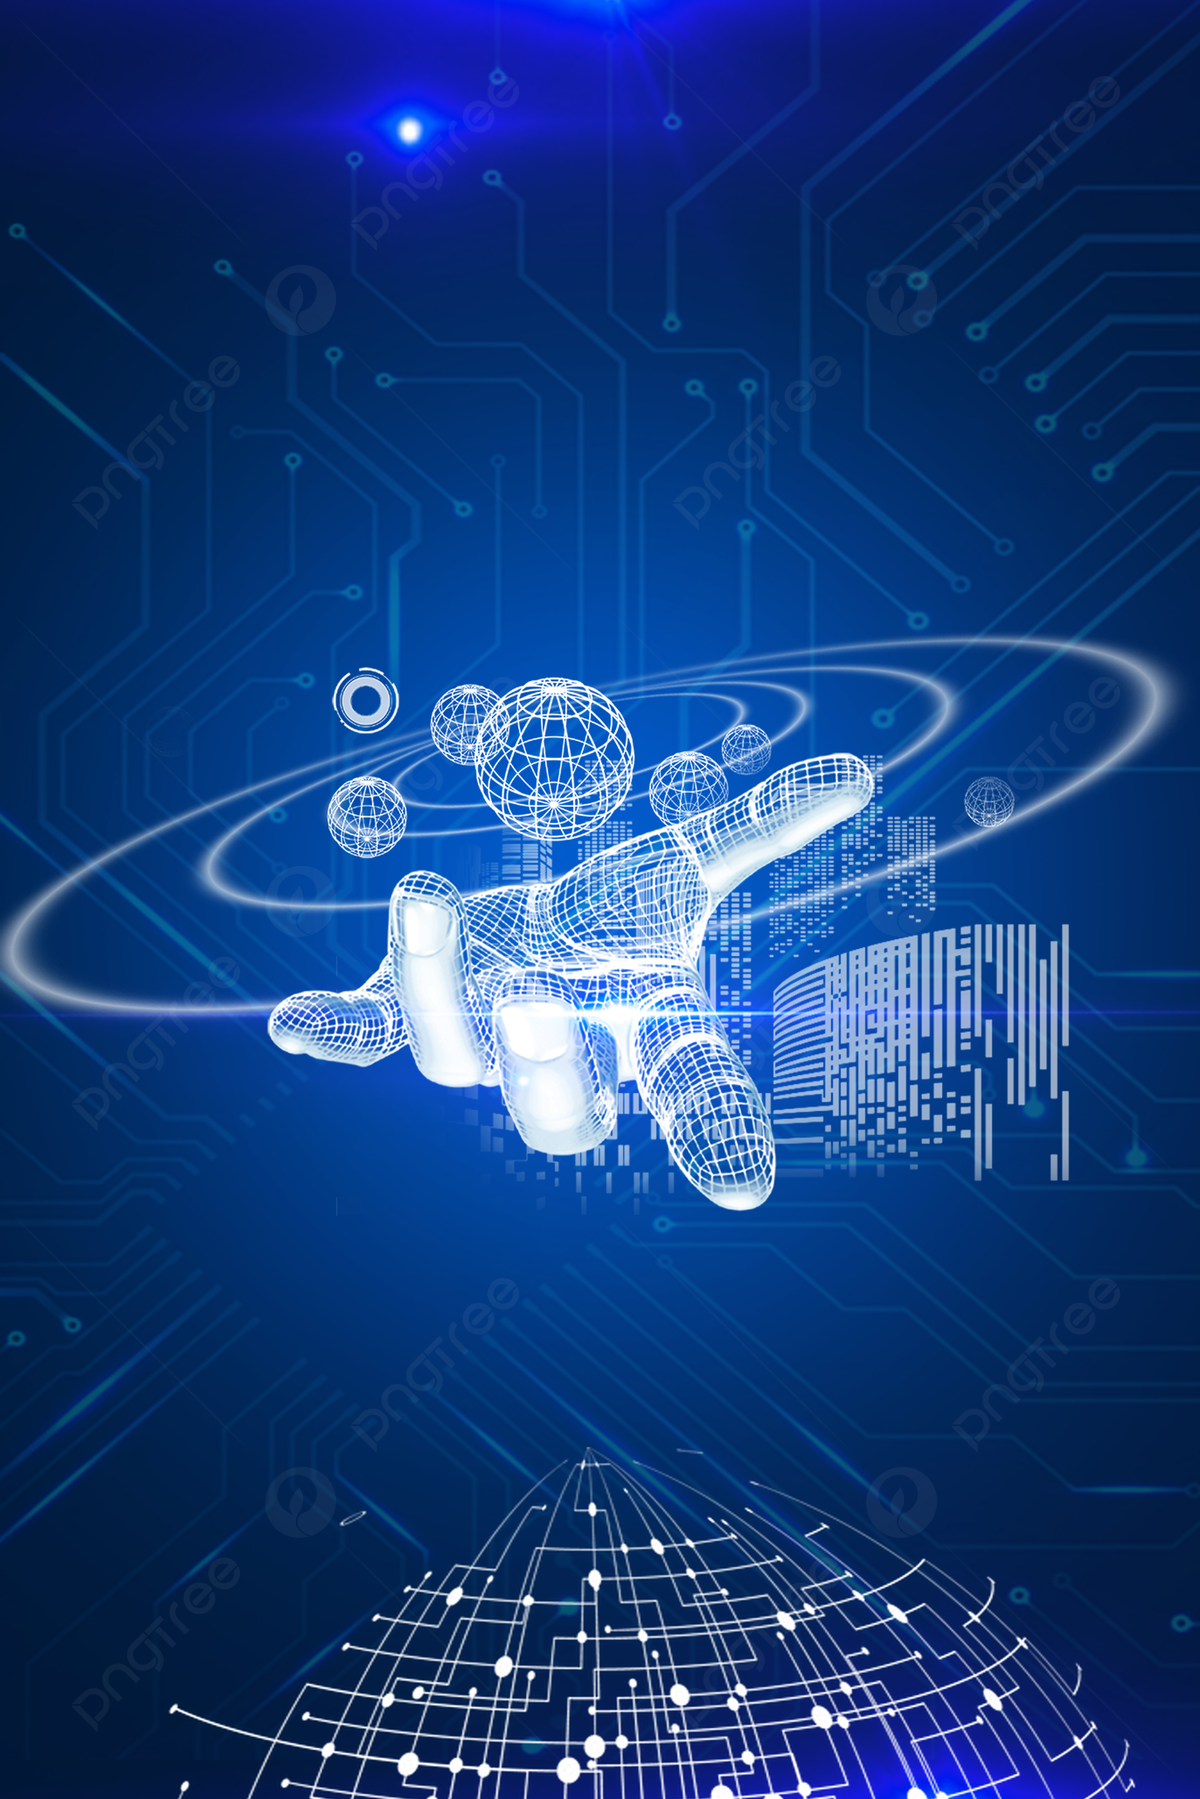
\includegraphics[width=\paperwidth,height=\paperheight]{portada.png}};
            \node[align=center] at (current page.center) {
                
                \vspace{0.5cm}
                \LARGE \textbf{Ismael Sallami Moreno} \\
                \LARGE \texttt{ism350zsallami@correo.ugr.es} \\
                \LARGE \url{https://ismael-sallami.github.io/} \\
                \LARGE \url{https://elblogdeismael.github.io/} \\
                \vspace{2cm}
                \Large \textbf{Universidad de Granada} \\
                \vspace{0.8cm}
                % \Large \textbf{2025}
            };
        \end{tikzpicture}
        \vfill
        
        \Large
        \textbf{2025}
        
    \end{center}
\end{titlepage}
\newpage


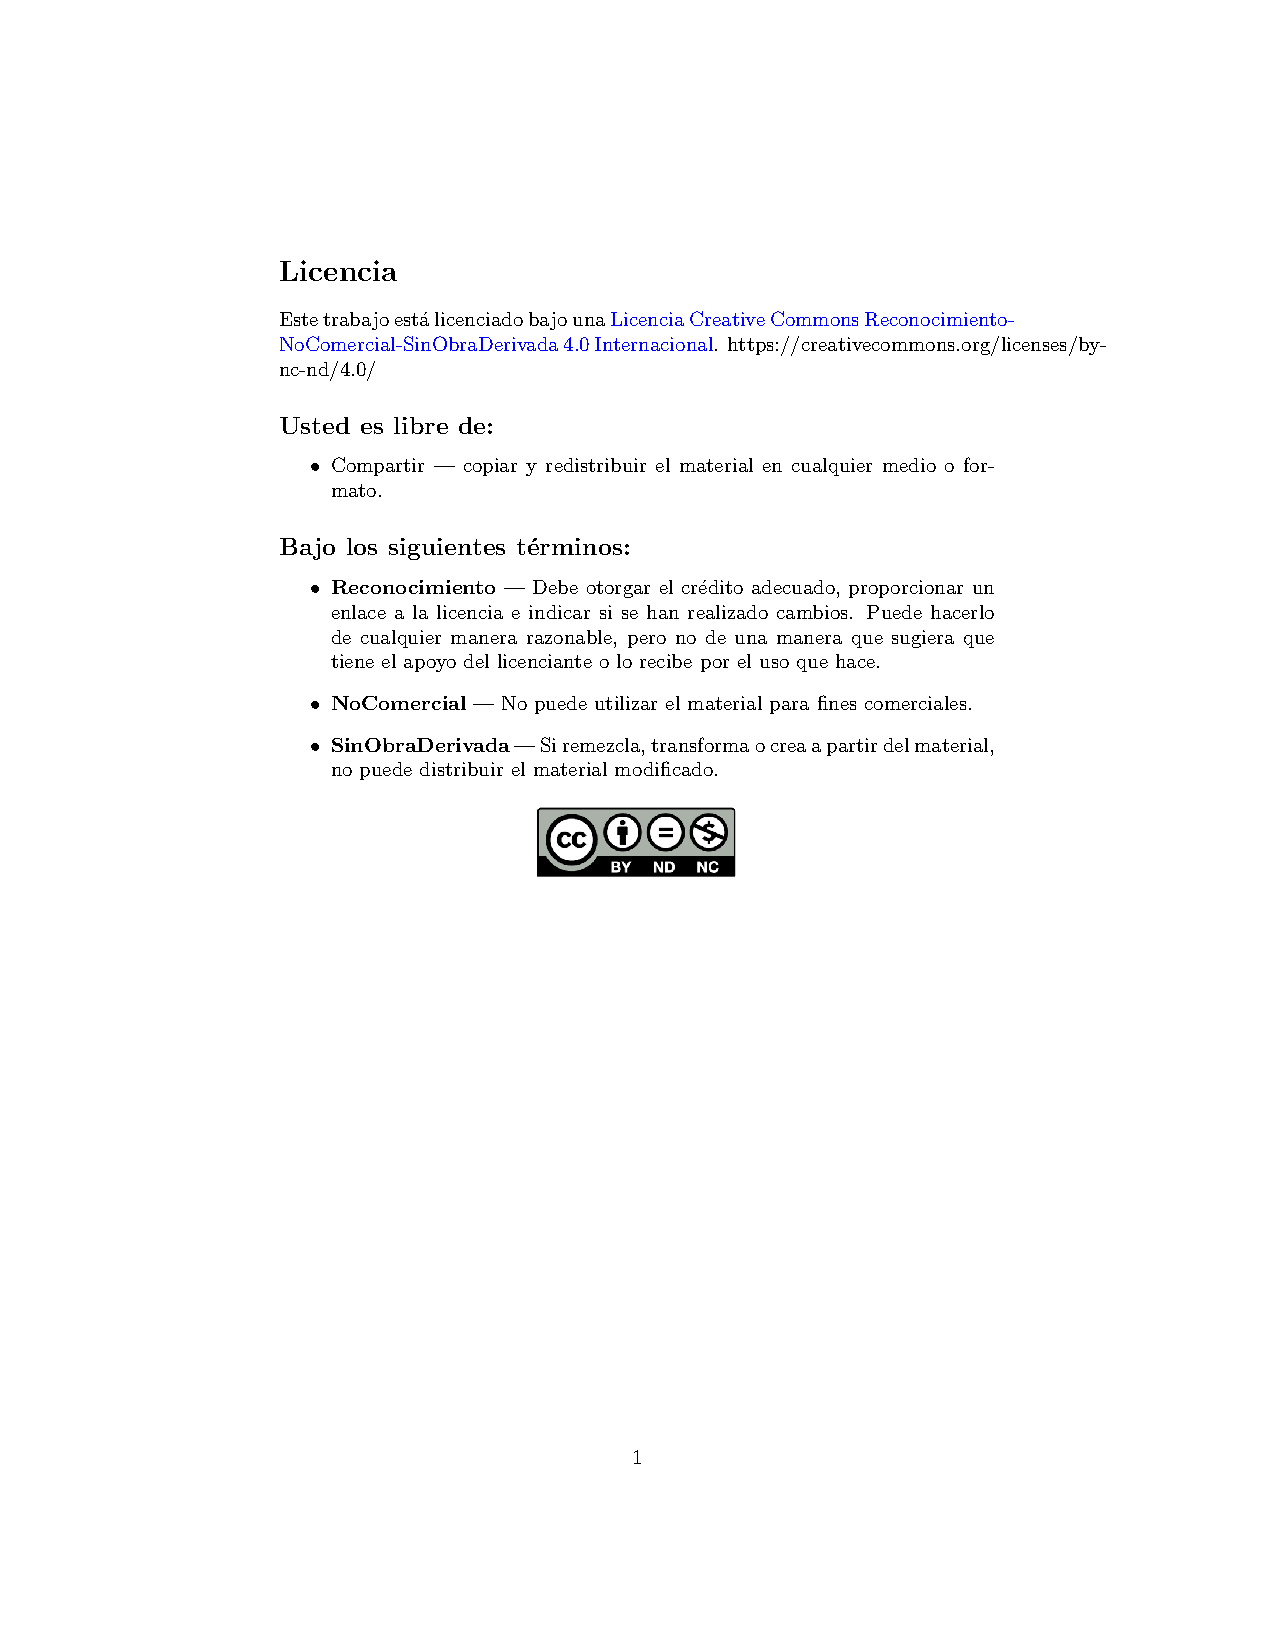
\includepdf[pages=-]{../../../../licencia.pdf}

% Tabla de contenidos
\tableofcontents
\newpage

% \chapter{Introducción}
% \section{Apuntes de CLase}
% \section{Introducción: Inteligente}
Debemos de definir la inteligencia artificial
usando la palabra inteligente, la cual es difícil de definir. Se dan diferentes definiciones de Harvard y otras universidades/entidades reconocidas. 

\section{Definición de IA}

Podemos tener varias definiciones de IA, como pueden ser sistemas que actúan/piensan como humanos, o bien sistemas que actúan/piensas racionalmente. Una de ellas puede ser: "Campo de estudio que busca explicar y emular el comportamiento inteligente en términos de procesos computacionales"

Un ejemplo de IA que menciona el profesor reiteradamente es el caso de los \textit{cajeros automáticos}.

\begin{tcolorbox}[colback=blue!20, colframe=blue]
Se garantiza que una pregunta sobre las definiciones de IA cae.
    
\end{tcolorbox}

Asociamos el concepto de IA a racional debido a que se quiere desarrollar con la capacidad de poder tomar decisiones como los humanos.

Hay distintos softwares en los dispositivos que podemos relacionarlos con la acción de que \textit{piensan} debido a que usan inteligencia artifical, como es el caso de programas de ajedrez. ¿Es esto correcto? No podemos afirmar esto exactamente, ya que según autores pensar es emular la mente humana, cosa que no es capaz de hacer la IA debido a que solo esta entrenado a hacer las mejores jugadas para ganarte, mientras que tu puedes pensar sobre otras temáticas y tener cierto \textit{pensamiento libre}.

Si afirmamos que piensan como humanos, debemos de tener en cuenta el \textit{pensamiento cognitivo}.

La IA según el libro del \textit{Porque} (recibió el premio Turing), tiene 3 niveles:
\begin{enumerate}
    \item Aprendizaje automático.
    \item Simular al humano.
    \item Capacidad de imaginar, lo cual, a día de hoy es inalcanzable.
\end{enumerate}

En cuanto a la creatividad, hay cierta\textit{ creatividad cognitiva }en temas específicos.

El llamado 'no alineamiento con los humanos' es lo que ocurre cuando una IA no tiene información sobre ese tema o bien no esta entrenado, pues en este caso se lo inventa.

El Test de Turing, es aquel en el que si una IA consigue pasar desapercibido como humano, pues efectivamente pasa este Test.

En esta asignatura vamos a seguir la Teoría del Agente, que es la idea más aceptada hoy día y más usada. Este percibe el entorno y actúa de una manera específica. 

Se usa la palabra \textit{racional} aludiendo a inteligente.

Un agente racional actúa de manera correcta según la información que posee.

El origen del término de IA recae en John McCarthy. Los pioneros de la IA son varios, entre los que podemos encontrar a Alan Turing, Marvin Minsky,...

En el debate de la IA se menciona una IA fuerte y una débil, que son sistemas que actúan como humanos y racionalmente vs las que piensan como IA.

En cuanto al recorrido de la IA a lo largo de la historia, podemos destacar distintas épocas como es la Edad de Oro, Invierno de IA,...

Von Neumann propone el algoritmo MiniMax, el que afirma que el juego es una situación conflictiva en la que tomamos decisiones sabiendo que los demás también las toman, determinando el resultado en base a las decisiones realizadas.
Un hecho histórico destacable, es que Napoleón murió pensando que había perdido jugando al ajedrez pensando que perdió frente al primer sistema inteligente, aunque puede que haya sido un humano. 
Otro de los avances importantes es el caso de los cohes autónomos.

En cuanto a los tipos de IA podemos mencionar:

\begin{itemize}
    \item IA débil: una máquina que compite con un humano en una actividad específica.
    \item IA fuerte: IA que aplica inteligencia para cualquier problema.
    \item IA general: alcanza el nivel cognitivo humano.
    \item Super-IA: capacidad que es mucho mayor que cualquier cerebro humano en cualquier campo.
\end{itemize}


%\chapter{Agentes}
% \section{Apuntes de CLase}
% \section{Concepto}
La Teoría de Agentes(denotado a continuación como \textbf{TA}) es un sistema de ordenador, situado en un entorno, capaz de realizar acciones de manera autónoma y que es flexible en base a las situaciones que se le presentan.

\section{Agentes Inteligentes}

Desarrolla un enfoque basado en agentes y lleva a cabo percepciones procesada mediante algoritmos de análisis y toma de decisiones. 
La TA se usa actualmente en la mayoría de ámbitos y es lo que más se usa hoy en día.

En cuanto a los tipos de agentes encontramos:

\begin{itemize}
    \item Reactivo: reacciona en base al entorno.
    \item Pro-activo: no solo actúan en respuesta al entorno, sino que puedan analizar acciones a llevar a cabo.
    \item  Social: son además capaces de interactuar.
    \item Multiagente: esta implementado como varios agentes interactuando.
\end{itemize}

La interacción entre agentes se lleva a cabo mediante: cooperación, coordinación y la negociación.


\section{Arquitecturas de Agentes}

Podemos distinguir entre:

\begin{itemize}
    \item Reactivo: reacciona en base a la situación en la que se encuentra, eligiendo la más adecuada en base a lo que sabe.
    \item Deliberativo: toma decisiones basadas en razonamiento, planificación y modelos internos del mundo.
\end{itemize}

Ya se puede hablar del concepto de Sistema de IA. El primer paso es el diseño del algoritmo. Cuando se lleva al campo de implementación, hablamos de Modelo de IA. Usamos datos para poder entrenar el modelo. Fianalmente, tengo un sistema de IA\footnote{Entendemos por sistema al resultado final que obtenemos tras la implementación y el entrenamiento del modelo.}.

Un término que se esta usando actualmente por las grandes empresas, es el concepto de Agente de IA, que es el sistema que se usa para realizar una determinada tarea, como es el caso de un doctor de turno.

\subsection{Concepto de Agente Inteligente}

Se trata de un sistema de ordenador, situado en un entorno, capaz de realizar acciones de forma \textit{autónoma} y que es \textit{flexible}. Trata la \textit{situación} en la que se encuentra.
Además debemos de tener en cuenta la caterística de transparencia, es decir, que el agente sea capaz de explicar el por qué de sus acciones. Solo es autónomo en entornos que considere seguro.

\begin{figure}[H]
    \centering
    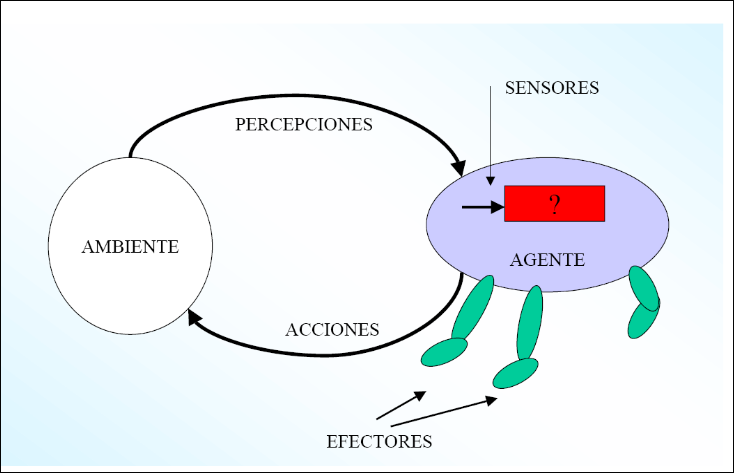
\includegraphics[width=0.5\textwidth]{images/Tema2/metodo.png}
    \caption{Método de reacción de un agente.}
    \label{fig:agentes}
\end{figure}

Ejemplo de estas percepciones, puede ser, para detectar el cáncer en alguna de las partes del cuerpo, se usan agentes que detectan la presencia de células cancerígenas en base a las imágenes del tumor.

Los agentes ofrecen una perspectiva innovadora
para representar la Inteligencia Artificial,
permitiendo abordar sus diversas áreas desde
un enfoque basado en agentes que ejecutan
acciones en función de percepciones procesadas
a través de mecanismos avanzados de análisis y
toma de decisiones.

Tema que cabe destacar, es que qen cuanto a la regulación de la IA, aún no esta decidida, si nos ponemos en el caso de que una IA causa algún daño, ¿quién es el responsable? ¿El creador de la IA o la IA en sí? Aún no se puede responder a esta pregunta.

Cuando tratamos el concepto de flecibilidad nos referimos a que sea capaz de realizar acciones de forma autónoma y que es
flexible para lograr los objetivos planteados.
\begin{itemize}
    \item Reactivo: reacciona en base al entorno.
    \item Pro-activo: no solo actúan en respuesta al entorno, sino que puedan analizar acciones a llevar a cabo.
    \item Social: son además capaces de interactuar con otros agentes.
\end{itemize}

Una \textit{nota imporatante} es el caso de GoogleMaps, ya que es deliberativo, pero esta diseño en cuanto a Software es reactivo.

Además, debemos de conocer el concepto de Sistema Multiagente, que es un sistema que se implementa como varios agentes interactuando entre sí, y de esta manera se consiguen numerosas versiones para resolver un problema.

Estos deben de ser capaces de cooperar, coordinarse y negociar entre ellos.

\subsection{IA Distribuida}

Destacamos los conceptos:
\begin{itemize}
    \item SMA: red más o menos unida de resolutores para solucionar problemas que solos sería más difícil.
    \item Resolutor: agente autónomo y de naturaleza heterogénea.
\end{itemize}

\subsubsection{Características}

Tiene información incompleta, no hay un sistema de control global, los datos no están centralizados y la computación es asincrónica.

\subsection{Arquitecturas de Agentes}

Podemos encontrarnos con las arquitecturas deliberativas y reactivas.

\subsubsection{Deliberativas}

Podemos encontrar un sistema de símbolso físicos, que es un conjunto de entidades físicas que pueden combinarse para formar estructuras más complejas. Se basa en la lógica y en la representación del conocimiento. Existe una \textit{hipótesis de sistema de símbolos inteligentes}, la cual dice qeu estos son capaces de generar acciones inteligentes.

Conocemos por \textit{Agente deliberativo} a  aquel que contiene un modelo simbólico del
mundo explícitamente representado, y cuyas decisiones se realizan a
través de un razonamiento lógico basado en emparejamientos de
patrones y manipulaciones simbólicas. Evalúa diferentes opciones de
acción considerando sus objetivos y selecciona la acción que
considera más adecuada según su razonamiento lógico.

Sabemos que toman decisiones en base a un razonamiento lógico, planificación y modelos internos del mundo.

Tenemos un problema: problema de representar simbólicamente la
información acerca de entidades y procesos
complejos del mundo real, y como conseguir que los
agentes razonen con esta información para que los
resultados sean útiles.

Como \textit{Ejemplo de agente deliberativo}, debemos de mencionar al problema del viajante del comercio, visto en otras Asignaturas como Algorítmica o Métodos Cuantitativos.
Este problema consiste en encontrar la ruta más corta que pasa por todas las ciudades y vuelve a la ciudad de origen.

\subsubsection{Reactivas}

Estos agentes reaccionan a la situación en la que se encuentran, eligiendo la acción más adecuada en base a lo que saben. No tienen un modelo interno del mundo, sino que reaccionan a la situación en la que se encuentran. Por lo que podemos decir que no hacen uso del razonamiento lógico.

\begin{figure}[H]
    \centering
    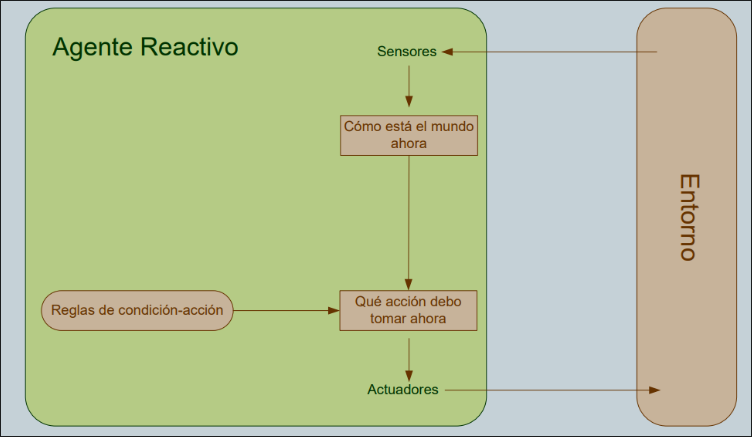
\includegraphics[width=0.7\textwidth]{images/Tema2/ar_re.png}
    \caption{Arquitectura reactiva.}
    \label{fig:reactivo}
\end{figure}

Uno de los ejemplos ed los agentes reactivos es \textit{es el robot que recorre un pasillo y evita obstáculos}. Este robot no tiene un modelo interno del mundo, sino que reacciona a la situación en la que se encuentra.

\subsubsection{Arquitecturas Híbridas}

Encontramos una estructura compuesta por capas reactivas y deliberativas. La capa reactiva se encarga de la percepción y la acción, mientras que la capa deliberativa se encarga de la planificación y el razonamiento. Tenemos una entrada sensorial, que se encarga de la percepción, y una salida motora, que se encarga de la acción.

Agente racional es similar a Agente inteligente.

En base a una serie de factores, podems definir un agente racional como: en cada posible secuencia de percepciones, un agente racional debe de seleccionar una acción que maximice su rendimiento, en base a la evidencia proporcionada por la secuencia de percepciones y en base al conocimiento que posee.

\subsection{Agentes Reactivos}

La característica principal de un agente reactivo es
su capacidad de responder directamente a estímulos
del entorno sin recurrir a un modelo interno o un
proceso de planificación. Este tipo de agente actúa
de manera inmediata basándose en reglas
predefinidas que relacionan percepciones con
acciones, lo que lo hace eficiente en entornos
dinámicos, aunque limitado en situaciones que
requieran razonamiento complejo.

En cuanto a las representaciones del mundo, podemos encontrar los módelos icónicos y los modelos basados en Características.

\subsubsection{Percepción y Acción}

El agente mediante estímulos a través de sensores, procesa la información, escoge una acción y la lleva a cabo mediante actuadores.

\begin{figure}[H]
    \centering
    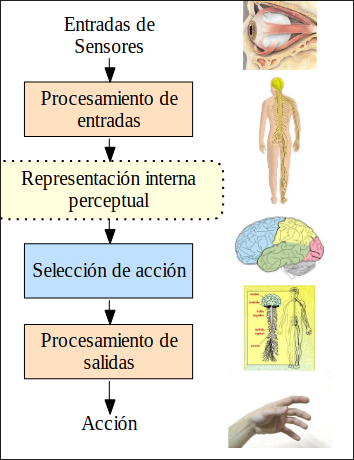
\includegraphics[width=0.4\textwidth]{images/Tema2/percep.png}
    \caption{Método de reacción de un agente.}
    \label{fig:agentes}
\end{figure}

\subsubsection*{Ejemplo del Diselo de un Agente Reactivo}
\begin{itemize}
    \item Ejemplo:
    \begin{itemize}
        \item Supongamos un robot en un mundo dividido en cuadrículas.
        \item El robot puede percibir si las 8 casillas vecinas están libres o no, con un sensor si por cada casilla i.
        \item El objetivo del robot es ir a una pared y seguir su perímetro indefinidamente.
        \item Tiene 4 posibles movimientos (de 1 casilla cada uno): Ir a Norte, Sur, Este u Oeste.
        \item No se permite que el entorno contenga pasillos estrechos (aquellas casillas rodeadas por dos o más obstáculos a ambos lados).
    \end{itemize}
\end{itemize}

Para verlo en detalle, ver las diapositivas 40-44.

\begin{itemize}
    \item Sistema de Producción: es un sistema de reglas que relacionan percepciones con acciones.
    \item Redes: son sistemas de reglas que se activan en paralelo.
    \item Arquitectura de subsunción: consiste en agrupar módulos de comportamiento en capas, donde cada capa tiene prioridad sobre la anterior. Cada módulo de comportamiento tiene una
    acción asociada, recibe la percepción
    directamente y comprueba una condición. Si esta
    se cumple, el módulo devuelve la acción a
    realizar.
    Un módulo se puede subsumir en otro. Si el
    módulo superior del esquema se cumple, se
    ejecuta este en lugar de los módulos inferiores.
\end{itemize}

\subsubsection{Agentes Reactivos con memoria}

Tiene ciertas limitaciones en cuanto al sistema sensorial, pero mejorar la precisión teniendo en cuenta la información previa.

Conocemos por \textit{Agente reactivo con memoria} a aquel que, además de reaccionar a la situación en la que se encuentra, tiene en cuenta información previa para mejorar la precisión de sus acciones.

Características de Agentes Reactivos:

\begin{itemize}
    \item Se diseñan completamente y por tanto es necesario anticipar todas
    las posibles reacciones para todas las situaciones.
    \item Realizan pocos cálculos y por tanto son rápidos.
    \item No tienen capacidad de aprendizaje.
    \item Almacenan todo en la memoria.
\end{itemize}

\begin{tcolorbox}[colback=yellow!10!white, colframe=yellow!90!black, title=¿Qué tipo de agente es ChatGPT?]
ChatGPT es un agente deliberativo, ya que utiliza un
proceso interno para generar respuestas basadas en
entradas del usuario, un vasto modelo de
conocimiento, y razonamiento complejo. Evalúa el
contexto y decide la mejor "acción" (respuesta) a
través de un procesamiento reflexivo y estructurado.
Sin embargo, también puede presentar características
reactivas, ya que responde rápidamente a estímulos
(mensajes) sin requerir planificación a largo plazo. Por
lo tanto, combina elementos deliberativos con un alto
grado de eficiencia reactiva. (Respuesta de Copilot).
\end{tcolorbox}

\begin{tcolorbox}[colback=red!10!white, colframe=red!90!black, title=Advertencia]
Solo es materia de examen las diapositivas que no tienen el título en rojo, que son las que tenemos todos los grados.
\end{tcolorbox}
%\section{Relacion de Problemas 1}
%\documentclass[a4paper,12pt]{book}

% Paquetes necesarios
\usepackage[utf8]{inputenc}   % Codificación de caracteres
\usepackage[spanish]{babel}   % Idioma español
\usepackage[T1]{fontenc}      % Codificación de fuentes
\usepackage{amsmath, amssymb} % Símbolos matemáticos
\usepackage{graphicx}         % Inclusión de gráficos
\usepackage{cite}             % Gestión de citas
\usepackage{hyperref}         % Enlaces y referencias
\usepackage{geometry}         % Configuración de márgenes
\usepackage{fancyhdr}         % Encabezados y pies de página
\usepackage{titlesec}         % Formato de títulos
\usepackage{booktabs}         % Tablas profesionales
\usepackage{caption}          % Personalización de leyendas
\usepackage{enumitem}         % Personalización de listas
\usepackage{float}
\usepackage{tcolorbox}
\usepackage[table]{xcolor} % Paquete para colores en tablas
\usepackage{colortbl}       % Complemento para colorear celdas específicas
\usepackage{multirow}       % Combinar celdas en tablas
\usepackage{makecell}       % Combinar celdas en tablas
\usepackage{enumitem}
\usepackage{amsmath}
\usepackage{eurosym}
\usepackage{tikz}
\usepackage{listings}
\usepackage{color}
\usepackage{float}
\usepackage{pdfpages}
% Configuración de márgenes
\geometry{left=3cm, right=3cm, top=2.5cm, bottom=2.5cm}

% Configuración de encabezados y pies de página
% \setlength{\headheight}{14.49998pt}
\pagestyle{fancy}
\fancyhf{}
\fancyhead[L]{Universidad de Granada}
\fancyhead[L]{\nouppercase{\leftmark}}

% \fancyhead[C]{Escuela Técnica Superior de Ingenierías Informática}
\fancyhead[R]{Fundamentos de Base de Datos}
\fancyfoot[L]{\rule[0pt]{\textwidth}{0.2pt}\\Ismael Sallami Moreno}
\fancyfoot[C]{\rule[0pt]{\textwidth}{0.2pt}\\\thepage}
\fancyfoot[R]{\rule[0pt]{\textwidth}{0.2pt}\\\today}
\renewcommand{\sectionmark}[1]{\markboth{#1}{}} % Configura \leftmark para que solo muestre la sección


% Formato de títulos
\titleformat{\section}{\large\bfseries}{\thesection.}{0.5em}{}
\titleformat{\subsection}{\normalsize\bfseries}{\thesubsection.}{0.5em}{}

% Datos del documento
\title{\textbf{Temario Inteligencia Artificial}}
\author{
    Ismael Sallami Moreno \\
    \texttt{ism350zsallami@correo.ugr.es}
}
\date{
    \vspace{1cm}
    \begin{tabular}{rl}
        \textbf{Asignatura:} & Fundamentos de Base de Datos \\
        \textbf{Tema:} & Teoría \\
        \textbf{Fecha:} & \today
    \end{tabular}
}

% Comando para definir código en línea que se muestra en cursiva y no se sale del PDF
\newcommand{\inlinecode}[1]{\texttt{\textit{#1}}}


\begin{document}

% Portada
\begin{titlepage}
    \begin{center}
        % \vspace*{1cm}
        
        % \Huge
        % \textbf{Práctica Contabilidad Financiera II}
        \Huge \textbf{FBD - Relación de Ejercicios Tema 1: Introducción y definiciones iniciales} 
        % \vspace{0.5cm}
        % \LARGE
        % \textbf{Ismael Sallami Moreno}\\
        % \LARGE
        % \texttt{ism350zsallami@correo.ugr.es}
        % \LARGE
        % \url{https://github.com/Ismael-Sallami}
        
        % \vfill
        
        % \Large
        % \textbf{Universidad de Granada}
        
        \vspace{0.8cm}
        
        \begin{tikzpicture}[remember picture, overlay]
            \node[opacity=0.2] at (current page.center) {
\includegraphics[width=\paperwidth,height=\paperheight]{portada.jpg}};
            \node[align=center] at (current page.center) {
                
                \vspace{0.5cm}
                \LARGE \textbf{Ismael Sallami Moreno} \\
                \LARGE \texttt{ism350zsallami@correo.ugr.es} \\
                %\LARGE \url{https://ismael-sallami.github.io/} \\
                %\LARGE \url{https://elblogdeismael.github.io/} \\
                \vspace{2cm}
                \Large \textbf{Universidad de Granada} \\
                \vspace{0.8cm}
                % \Large \textbf{2025}
            };
        \end{tikzpicture}
        \vfill
        
        \Large
        \textbf{2025}
        
    \end{center}
\end{titlepage}
\newpage


%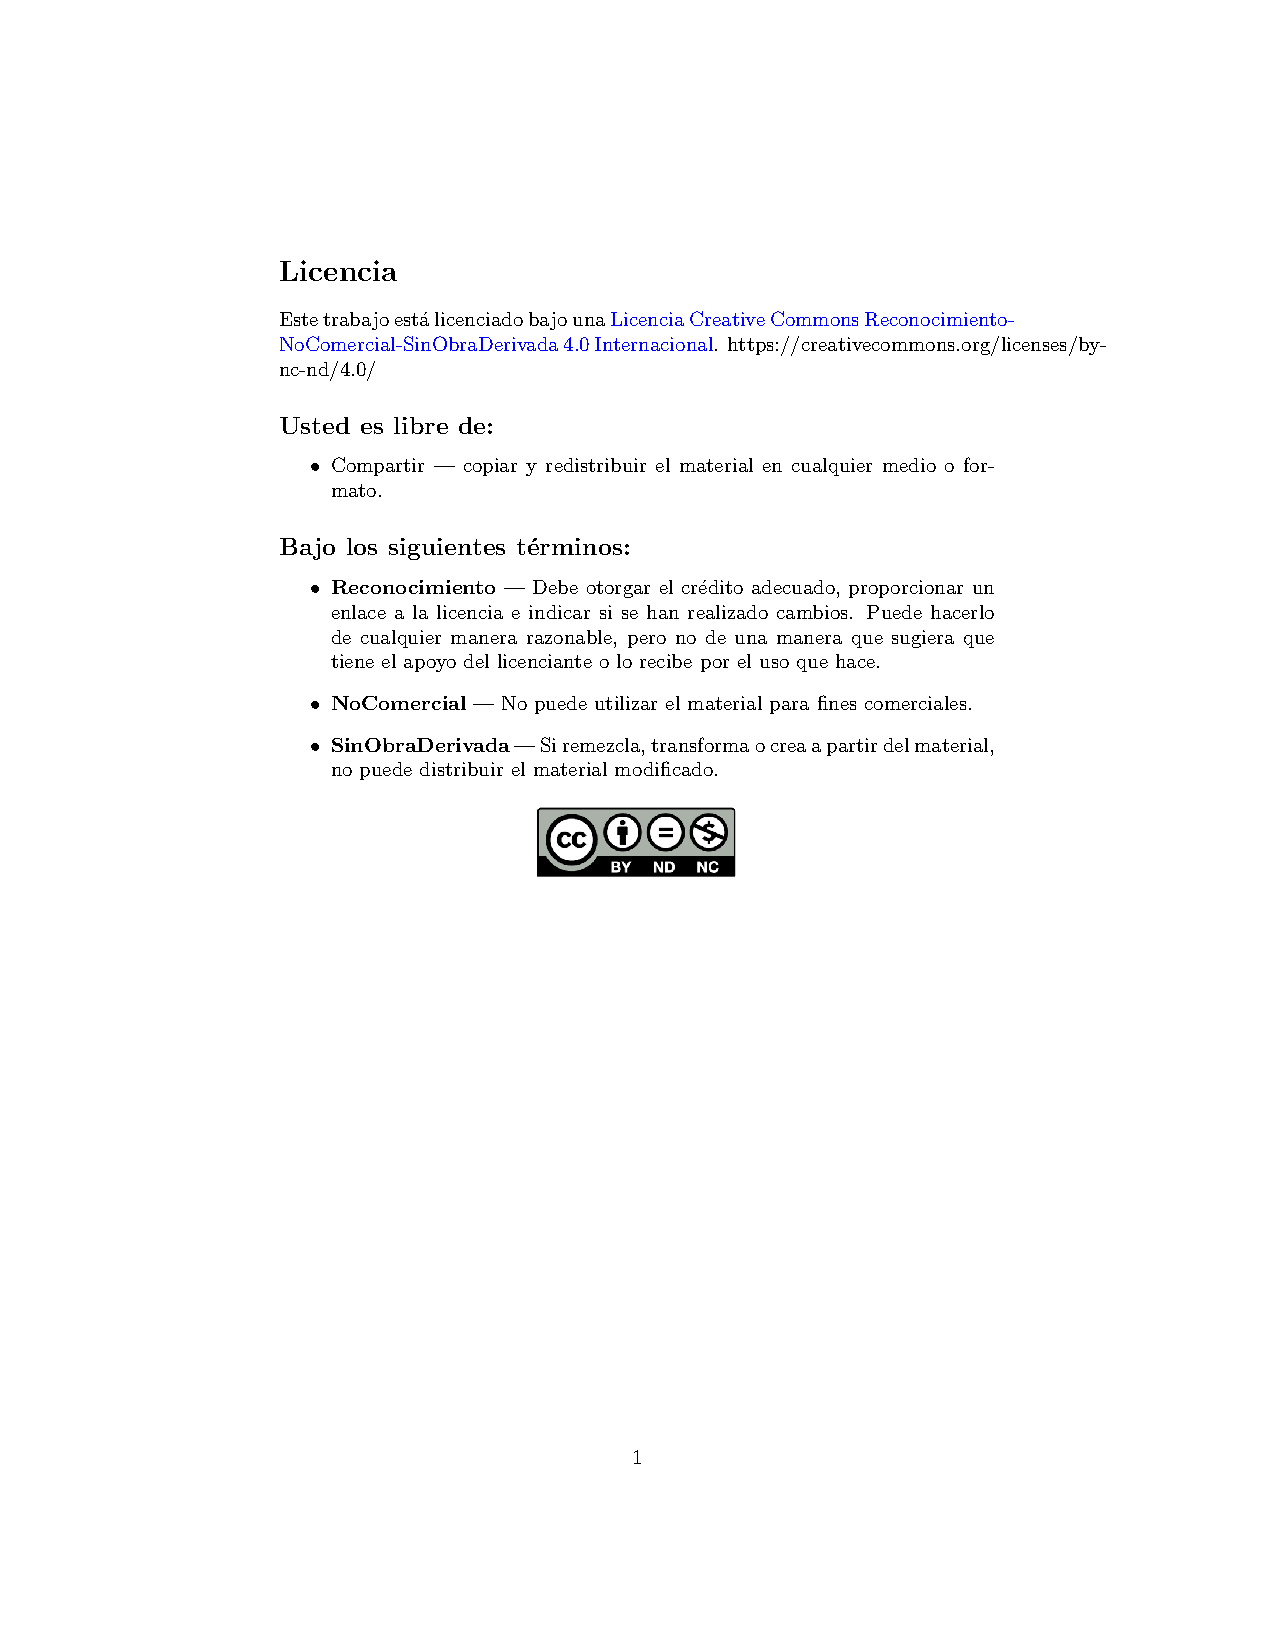
\includepdf[pages=-]{../../../../licencia.pdf}
% Tabla de contenidos
\tableofcontents
\newpage

\chapter{Introducción y definiciones iniciales}

\section{Introducción}
Este es un documento de prueba en \LaTeX. Aquí puedes escribir el contenido de tu primer capítulo.

\section{Definiciones Básicas}
\subsection{Definición 1}
Una definición básica para comenzar:
\[
E = mc^2
\]
donde $E$ es la energía, $m$ es la masa y $c$ es la velocidad de la luz.

\subsection{Definición 2}
Otra definición importante:
\[
a^2 + b^2 = c^2
\]
que corresponde al teorema de Pitágoras.

\section{Conclusión}
Este es un ejemplo básico de cómo estructurar un capítulo en \LaTeX. Puedes expandirlo según tus necesidades.




\newpage
% Referencias
\begin{thebibliography}{99}
\bibitem{Referencia1}
Ismael Sallami Moreno, \textbf{Estudiante del Doble Grado en Ingeniería Informática + ADE}, Universidad de Granada, 2025.
% \bibitem{Referencia2}
% Autor(es), \emph{Título del libro}, Editorial, año.

% \bibitem{Referencia3}
% Autor(es), \emph{Título del documento}, Nombre de la Conferencia, páginas, año.
\end{thebibliography}

\end{document}


%\chapter{Búsqueda en espacios de estados}
%\section{Problema del mono y el plátano}

\subsection*{Descripción del Problema}
Un mono se encuentra en la puerta de una habitación. En el centro de la habitación hay un plátano colgado del techo, pero el mono no puede alcanzarlo desde el suelo. En la ventana de la habitación hay una caja que el mono puede mover y sobre la que puede subirse para alcanzar el plátano.

\subsection*{Acciones Disponibles}
El mono puede realizar las siguientes acciones:
\begin{itemize}
    \item Desplazarse entre la puerta, el centro y la ventana.
    \item Empujar la caja mientras se mueve.
    \item Subirse a la caja.
    \item Coger el plátano.
\end{itemize}

\subsection*{Representación de Estados}
El estado se representa mediante una tupla $(X, Y, W, Z)$ donde:
\begin{itemize}
    \item $X$: Posición del mono en la habitación (\texttt{puerta}, \texttt{centro}, \texttt{ventana}).
    \item $Y$: Situación del mono respecto a la caja (\texttt{suelo}, \texttt{caja}).
    \item $W$: Posición de la caja en la habitación (\texttt{puerta}, \texttt{centro}, \texttt{ventana}).
    \item $Z$: Posesión del plátano (\texttt{tiene}, \texttt{no\_tiene}).
\end{itemize}
\newpage
\subsection*{Solución}
La secuencia de acciones para que el mono consiga el plátano es la siguiente:

\begin{enumerate}
    \item Estado inicial:
    \begin{equation}
    \text{estado}(\text{puerta}, \text{suelo}, \text{ventana}, \text{no\_tiene})
    \end{equation}
    
    \item Andar a la ventana:
    \begin{equation}
    \text{estado}(\text{ventana}, \text{suelo}, \text{ventana}, \text{no\_tiene})
    \end{equation}
    
    \item Empujar la caja al centro:
    \begin{equation}
    \text{estado}(\text{centro}, \text{suelo}, \text{centro}, \text{no\_tiene})
    \end{equation}
    
    \item Subir a la caja:
    \begin{equation}
    \text{estado}(\text{centro}, \text{caja}, \text{centro}, \text{no\_tiene})
    \end{equation}
    
    \item Coger el plátano:
    \begin{equation}
    \text{estado}(\text{centro}, \text{caja}, \text{centro}, \text{tiene})
    \end{equation}
\end{enumerate}

Con esta secuencia de acciones, el mono logra su objetivo de obtener el plátano.



% \chapter{Búsqueda en Espacios de Estados}
% \section{Apuntes de CLase}
% \subsection{Diseño de un agente deliberativo: búsqueda en espacios de estados}

El agente dispone de un modelo del mundo donde actúa, modelo de efectos de las acciones sobre el mundo, es capaz de razonar sobre esos modelos para decidir que hacer para conseguir un objetivo.


Tras esta introducción, vamos a pasar a ver el espacio de estados.

\textbf{Espacio de Estados: } Representación del
conocimiento a través de las acciones del
agente.

\textbf{Búsqueda en Espacios de Estados: } Resolución del problema mediante proyección
de las distintas acciones.

Como ejemplo de agente deliberativo, se trata \textit{el problema del viajante de comercio}.



\newpage
% Referencias
\begin{thebibliography}{99}
\bibitem{Referencia1}
Ismael Sallami Moreno, \textbf{Estudiante del Doble Grado en Ingeniería Informática + ADE}, Universidad de Granada, 2025.
% \bibitem{Referencia2}
% Autor(es), \emph{Título del libro}, Editorial, año.

% \bibitem{Referencia3}
% Autor(es), \emph{Título del documento}, Nombre de la Conferencia, páginas, año.
\end{thebibliography}

\end{document}
